\section{Benchmark, Metrics, and Methodology}
\label{sec:methodology}

% =============================================================================
\subsection{Benchmark}
\label{sec:methodology:benchmark}

% Pipeline figure for §3. Shows: cipher BLIF -> three representations ->
% fault campaign -> three measured metrics, plus a side branch for the FPGA
% evaluation. Self-contained tikz block; \input it from §3 inside a figure.

\begin{figure*}[tbp]
  \centering
  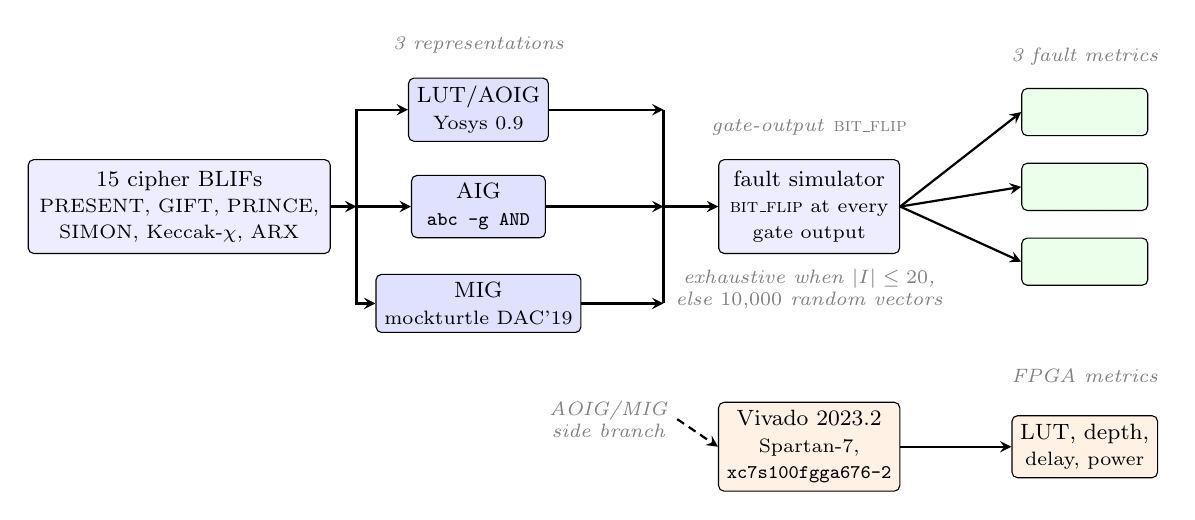
\begin{tikzpicture}[
    >=stealth,
    every node/.style={font=\footnotesize},
    block/.style={draw, rounded corners=2pt, minimum width=2.0cm,
                  minimum height=0.75cm, align=center, fill=blue!7,
                  inner sep=4pt},
    flow/.style={draw, rounded corners=2pt, minimum width=1.7cm,
                 minimum height=0.6cm, align=center, fill=blue!12,
                 inner sep=3pt},
    metric/.style={draw, rounded corners=2pt, minimum width=1.6cm,
                   minimum height=0.6cm, align=center, fill=green!8,
                   inner sep=3pt},
    fpga/.style={draw, rounded corners=2pt, minimum width=1.6cm,
                 minimum height=0.6cm, align=center, fill=orange!10,
                 inner sep=3pt},
    arrow/.style={->, thick},
    bus/.style={thick},
    note/.style={font=\scriptsize\itshape, gray},
  ]

    % ----- INPUT -----
    \node[block] (cipher) at (0, 0) {15 cipher BLIFs\\
        \scriptsize PRESENT, GIFT, PRINCE,\\
        \scriptsize SIMON, Keccak-$\chi$, ARX};

    % ----- THREE REPRESENTATIONS -----
    \node[flow] (aoig) at (3.8,  1.23) {LUT/AOIG\\\scriptsize Yosys 0.9};
    \node[flow] (aig)  at (3.8,  0.00) {AIG\\\scriptsize \texttt{abc -g AND}};
    \node[flow] (mig)  at (3.8, -1.23) {MIG\\\scriptsize mockturtle DAC'19};

    \coordinate (split) at (2.25, 0);
    \draw[arrow] (cipher.east) -- (split);
    \draw[arrow] (split) |- (aoig.west);
    \draw[arrow] (split) |- (aig.west);
    \draw[arrow] (split) |- (mig.west);

    % ----- COMMON FAULT CAMPAIGN -----
    \node[block] (sim) at (8.0, 0) {fault simulator\\
        \scriptsize \textsc{bit\_flip} at every\\
        \scriptsize gate output};

    \coordinate (faultbus) at (6.15, 0);
    \draw[bus] (faultbus |- aoig.east) -- (faultbus |- mig.east);
    \draw[arrow] (aoig.east) -- (faultbus |- aoig.east);
    \draw[arrow] (aig.east) -- (faultbus |- aig.east);
    \draw[arrow] (mig.east) -- (faultbus |- mig.east);
    \draw[arrow] (faultbus) -- (sim.west);

    % ----- METRICS -----
    \node[metric] (fc)   at (11.5,  1.2) {\FCpct};
    \node[metric] (avgdp) at (11.5, 0.25) {\AvgDP};
    \node[metric] (avgbw) at (11.5, -0.7) {\AvgBW};

    \draw[arrow] (sim.east) -- (fc.west);
    \draw[arrow] (sim.east) -- (avgdp.west);
    \draw[arrow] (sim.east) -- (avgbw.west);

    % ----- FPGA SIDE-CAMPAIGN -----
    \node[fpga] (vivado) at (8.0, -3.05) {Vivado 2023.2\\
        \scriptsize Spartan-7,\\
        \scriptsize \texttt{xc7s100fgga676-2}};
    \node[fpga] (fpga_metrics) at (11.5, -3.05) {LUT, depth,\\
        \scriptsize delay, power};

    \node[note, align=center] (fpga_src) at (5.45, -2.7)
      {AOIG/MIG\\side branch};
    \draw[arrow, densely dashed] (fpga_src.east) -- (vivado.west);
    \draw[arrow] (vivado.east) -- (fpga_metrics.west);

    % ----- LABELS -----
    \node[note] at (3.8, 2.05) {3 representations};
    \node[note] at (8.0, 1.0) {gate-output \textsc{bit\_flip}};
    \node[note] at (11.5, 1.9) {3 fault metrics};
    \node[note] at (11.5, -2.15) {FPGA metrics};

    % ----- TEST-VECTOR ANNOTATION -----
    \node[note, align=center] at (8.0, -1.05)
      {exhaustive when $|I| \le 20$,\\else $10{,}000$ random vectors};

  \end{tikzpicture}
  \caption{Measurement pipeline. Each of 15 cipher BLIFs is synthesized
  through three logical representations. The fault simulator injects a single \bitflip{}
  at every gate output of every netlist on every test vector
  (exhaustive when feasible; $10{,}000$ uniform random vectors
  otherwise), producing all-site and target-layer metrics
  (\FCpct{}, \AvgDP{}, \AvgBW). The FPGA side-branch reports LUT,
  depth, delay, and power for context on AOIG/MIG; the fault
  analysis is independent of FPGA tooling.}
  \label{fig:pipeline}
\end{figure*}

Fig.~\ref{fig:pipeline} sketches the full measurement pipeline.

We selected 15 cipher primitives spanning six architecture families:
four 4-bit S-boxes (PRESENT, GIFT, PRINCE, PRINCE$^{-1}$); three
substitution round functions (GIFT \texttt{subcells}, GIFT round,
PRESENT round); one permutation primitive (PRINCE $M'$); two SIMON
round functions (SIMON-32, SIMON-64); two Keccak-$\chi$ widths
(5-bit, 64-row); and three ARX primitives (Speck-32, SpecKey,
MARX-2). Input width ranges from 4 to 1280 bits. FPGA-oriented
AOIG/MIG metrics are included in the artifact for context, but
the fault-analysis claims below use the BLIF-level campaigns.

We analyze three logical representations, all derived from the same raw
cipher BLIF. \emph{LUT/AOIG} is the raw BLIF emitted by Yosys 0.9 from
the cipher's behavioral description, dominated by LUT-style truth-table
primitives. \emph{AIG} is a decomposed 2-input AND-inverter graph, used as a
comparable small-gate granularity control.
\emph{MIG} is a strict 3-input majority-inverter network produced with
the mockturtle logic-synthesis library~\cite{soeken2018mockturtle}. The
exact passes for the AIG and MIG flows are given in
\S\ref{sec:methodology:recipes}; the raw BLIFs and the synthesis driver
are in the artifact.

% =============================================================================
\subsection{Synthesis recipes}
\label{sec:methodology:recipes}

Because our central claim is that fault metrics depend on the gate-level
representation, the exact transformation from the common source BLIF to
each representation is part of the methodology. All three start from the
identical Yosys-emitted truth-table BLIF.

\textit{AIG.} We decompose the source BLIF into a 2-input AND-inverter
graph with Yosys and ABC, using the script
\texttt{read\_blif; hierarchy -auto-top; flatten; proc; techmap; opt;
abc -g AND; opt\_clean; write\_blif}. The \texttt{abc -g AND} step maps
all logic onto 2-input \textsc{and} nodes with inverter edges; no
optimization beyond \texttt{opt}/\texttt{opt\_clean} is applied. This
control exists only to provide a comparable small-gate fault-site
population for comparison with the MIG.

\textit{MIG.} We read the source BLIF into a $k$-LUT network and convert
it to an MIG by NPN node resynthesis
(\texttt{node\_resynthesis} with \texttt{mig\_npn\_resynthesis}). We then
apply a fixed DAC'19-style majority optimization recipe implemented with
stock mockturtle passes~\cite{amaru2019synth}: algebraic depth rewriting,
MIG resubstitution, cut rewriting with MIG NPN resynthesis, and
refactoring. In the artifact, this recipe is selected with
\texttt{--mode=area --mig-flow=dac19\_compat}; the option is used only
to reproduce the mockturtle flow. The resulting netlists are strict
3-input majority-inverter graphs.

% =============================================================================
\subsection{Metrics}
\label{sec:methodology:metrics}

We measure \emph{fault observability}: after flipping one gate-output
bit, does any primary output change, and if so, how often and by how
many bits? This is not a full key-recovery metric. It is a gate-level
description of how injected faults reach the circuit outputs.

Let $C$ have primary inputs $I$, primary outputs $O$, and internal
signals $G(C)$. Let $\mathcal{P}$ be the test-vector set (exhaustive
when $|I| \le 20$, otherwise $10{,}000$ uniform random vectors with
fixed seed). For each fault site $g \in G(C)$ and each vector
$P \in \mathcal{P}$, let $\text{out}(P)$ denote the fault-free primary
outputs and $\text{out}_g(P)$ the primary outputs when $g$ is subject
to a single \bitflip{}. We report three metrics.

\textit{Fault coverage} \FCpct{} asks how many gate-output sites are
ever visible at the primary outputs. A site is detectable if at least
one tested vector makes the faulty output differ from the fault-free
output:
$|\{g : \exists P,\ \text{out}_g(P) \ne \text{out}(P)\}| / |G(C)|$.

\textit{Average per-vector detection probability} \AvgDP{} asks how
often a detectable site is visible. For a site $g$, $\text{dp}(g)$ is
the fraction of tested vectors on which flipping $g$ changes the
primary output. \AvgDP{} averages this value across detectable sites:
$\AvgDP(C) = \frac{1}{|\{g~\text{detectable}\}|} \sum_g \text{dp}(g)$,
where $\text{dp}(g) = |\{P : \text{out}_g(P) \ne \text{out}(P)\}| / |\mathcal{P}|$.
For example, if a fault changes the output on 8 of 16 exhaustive input
vectors, then $\text{dp}(g)=0.5$.

\textit{Average breadth} \AvgBW{} asks how large the visible corruption
is. For every event where the faulty output differs from the correct
output, we count the primary-output Hamming distance. \AvgBW{} is the
mean of those distances over all detecting events.

These metrics vary independently. A circuit can have higher \FCpct{}
than another while having lower \AvgDP{}: more fault sites are
theoretically observable, but each is observed on a smaller share of
input space.

For the granularity-controlled analysis, we compute each metric over two
fault-site populations. The \emph{all-site} population includes every
gate-output site in the representation. This is the common campaign
design, but it is representation-sensitive because decomposing one
Boolean function into many small gates changes both the number and
location of sites being averaged. The \emph{target-layer} population
includes only gates that directly drive primary outputs. This is not a
complete physical fault model, but it is a realizable combinational DFA
target layer and removes the interior-node mix introduced by different
decompositions. Full definitions are in the artifact's
\texttt{paper/metrics.md}.

% =============================================================================
\subsection{Fault model and simulator}
\label{sec:methodology:simulator}

We adopt a single-fault model: the adversary injects one
\bitflip{} at one gate-output wire of the combinational netlist per
evaluation and observes the resulting primary outputs. We do not
model multi-bit faults, transistor-level effects, glitch injection,
delay faults, or end-to-end key-recovery attacks; these are
out of scope.

Our simulator parses BLIF, builds per-gate truth-table lookups, and
evaluates the netlist on all $|\mathcal{P}|$ vectors as a single
vectorized \texttt{numpy.uint8} array. For each gate $g$, the
fault-free signal value $v_g(P)$ is computed once; the faulty
evaluation re-runs propagation with the override
$g \mapsto v_g(P) \oplus 1$. The campaign re-runs full propagation for
each fault site across all test vectors in a vectorized batch; for
the largest circuit (\texttt{keccak\_chi\_64row}, 1602 gates,
$10{,}000$ vectors) it completes in approximately one minute on a
single core.

% =============================================================================
\subsection{Granularity-controlled assessment procedure}
\label{sec:methodology:procedure}

The assessment has three checks. First, we compute all-site \AvgDP{}
for each representation and compare the same MIG netlists against both
the LUT/AOIG baseline and the decomposed-AIG baseline. Second, we
measure the Spearman rank association between all-site \AvgDP{} and
decomposition granularity (fault sites per primary output). Third, we
repeat the campaign on the target-layer population only. These checks
allow us to separate representation-dependent all-site behavior from
behavior that remains stable under controlled fault-site populations.
Results are reported in \S\ref{sec:results}.

% =============================================================================
\subsection{Mechanism: how masking arises}
\label{sec:methodology:mechanism}

The LUT-to-MIG \AvgDP{} change in \S\ref{sec:results:granularity}
has a concrete gate-level mechanism, but the mechanism is a site-mix
effect, not evidence that majority logic is intrinsically more
fault resistant. A \bitflip{} at the output of
gate $g$ is, by definition, observable at $g$ itself because the fault
and the output are the same wire. The question is whether the flipped
value reaches a primary output, which depends entirely on $g$'s
downstream consumers.

For a 3-input majority gate $h$ that consumes $g$ along with two
other inputs $a$ and $b$, the output of $h$ is $1$ iff at least two of
its three inputs are $1$. The vote is \emph{determined} by $a$ and
$b$ alone when $a = b$: $h$'s output is fixed at that shared value
regardless of the third input. We call this the \emph{non-controlling
pattern at $h$ relative to $g$}, in keeping with the ATPG term. When
the other two inputs disagree, $a \ne b$, the third input casts the
deciding vote, and a flip at $g$ propagates through $h$.

Under a uniform distribution over $h$'s other two inputs, the
non-controlling pattern holds with probability $\frac{1}{2}$.
A fault at $g$ that has no downstream consumer other than $h$ therefore
has $\text{dp}(g) = \frac{1}{2}$ in the limit. A LUT-style AOIG
representation often contributes one wide output-adjacent fault site
with $\text{dp}=1$, whereas MIG and AIG decompositions contribute many
interior sites whose downstream consumers can mask them. The all-site
average therefore changes when the representation changes. The central
question in \S\ref{sec:results:granularity} is whether the sign of that
change survives when the baseline is decomposed to comparable
granularity.

% =============================================================================
\subsection{Worked example}
\label{sec:methodology:trace}

We make the mechanism concrete on the \texttt{present\_sbox} MIG
netlist. Gate $g = \texttt{new\_n12}$ is a 3-input majority of
\texttt{pi1}, \texttt{pi2}, and an internal signal \texttt{new\_n11}.
$g$ has exactly one downstream consumer, $h = \texttt{new\_n15}$,
which is a 3-input majority over \texttt{new\_n10}, the complement of
$g$'s value, and \texttt{new\_n14}.
Figure~\ref{fig:masking-example} shows the structure;
Table~\ref{tab:masking-trace} enumerates the per-vector behavior.

% Worked masking example: present_sbox MIG
% Fault site g = new_n12 (MAJ3 of pi1, pi2, new_n11)
% Downstream gate h = new_n15 (MAJ3 of new_n10, ~new_n12, new_n14)
% g has exactly one consumer (h), so dp(g) is determined entirely by h's masking.

\begin{figure*}[tbp]
  \centering
  \begin{tikzpicture}[
    >=stealth,
    every node/.style={font=\small},
    gate/.style={draw, rounded corners=1pt, minimum width=1.6cm,
                 minimum height=0.7cm, fill=blue!8},
    fgate/.style={draw, rounded corners=1pt, minimum width=1.6cm,
                  minimum height=0.7cm, fill=red!10, draw=red!70},
    wire/.style={->, thick},
    inv/.style={circle, inner sep=0pt, minimum size=4pt, draw, fill=white},
  ]
    % Primary inputs feeding g
    \node (pi1)   at (-3.2,   1.0) {\scriptsize \texttt{pi1}};
    \node (pi2)   at (-3.2,   0.3) {\scriptsize \texttt{pi2}};
    \node (n11)   at (-3.2,  -0.4) {\scriptsize \texttt{new\_n11}};

    % Fault gate g
    \node[fgate] (g) at (-1.0, 0.3) {\textsc{maj3} $g$};
    \node[above=2pt of g, font=\scriptsize\itshape] {fault site};

    \draw[wire] (pi1) -- (g.west |- pi1);
    \draw[wire] (pi2) -- (g.west);
    \draw[wire] (n11) -- (g.west |- n11);

    % Other inputs to h
    \node (n10)   at (1.5,  1.0) {\scriptsize \texttt{new\_n10}};
    \node (n14)   at (1.5, -0.4) {\scriptsize \texttt{new\_n14}};

    % Downstream gate h (sole consumer of g)
    \node[gate] (h) at (3.8, 0.3) {\textsc{maj3} $h$};

    % Inverter bubble on g -> h edge (h treats g's contribution complemented)
    \node[inv] (bubble) at (2.7, 0.3) {};

    \draw[wire] (g.east) -- (bubble.west);
    \draw[wire] (bubble.east) -- (h.west);
    \draw[wire] (n10) -- (h.west |- n10);
    \draw[wire] (n14) -- (h.west |- n14);

    % Output
    \node (out) at (6.2, 0.3) {\scriptsize \texttt{new\_n15}};
    \draw[wire] (h.east) -- (out.west);

    % Annotation: masking rule
    \node[align=center, font=\scriptsize, draw=gray!50,
          rounded corners=2pt, fill=gray!5, inner sep=4pt]
      (note) at (2.4, -1.7)
      {When \texttt{new\_n10} $=$ \texttt{new\_n14} (agree): non-controlling pattern, fault masked.\\[-1pt]
       When \texttt{new\_n10} $\neq$ \texttt{new\_n14} (disagree): fault propagates. (8\,/\,16 each.)};
    \draw[densely dotted, gray!70] (h) -- (note);
  \end{tikzpicture}
  \caption{Worked masking example from the \texttt{present\_sbox} MIG.
    Gate $g$ (fault site) feeds a single downstream MAJ3 gate $h$
    through a complemented edge. A bit-flip at $g$ propagates to $h$'s
    output iff the other two inputs of $h$ \emph{disagree}; when they
    \emph{agree}, they form the non-controlling pattern and mask the
    fault. Over the 16 exhaustive input vectors, the other two inputs
    agree on 8 vectors (fault masked) and disagree on 8 (fault propagates). Because $g$ has $h$ as its sole consumer, this
    completely determines $g$'s observability: $\mathrm{dp}(g) = 8/16
    = 0.5$. The per-vector trace in Table~\ref{tab:masking-trace}
    enumerates all 16 vectors.}
  \label{fig:masking-example}
\end{figure*}

% Summary of the exhaustive per-vector masking trace for present_sbox.

\begin{table}[tbp]
  \centering
  \caption{Worked-example trace summary. The fault at $g$ is masked when
  the other two inputs of $h$ agree and propagates when they disagree.}
  \label{tab:masking-trace}
  \footnotesize
  \setlength{\tabcolsep}{3.5pt}
  \begin{tabular}{@{}p{0.29\columnwidth}c p{0.28\columnwidth}p{0.23\columnwidth}@{}}
    \toprule
    Other inputs of $h$ & Vectors & Effect at $h$ & Outcome \\
    \midrule
    Agree, $a=b$ &
    $8/16$ &
    Output fixed by $a,b$ &
    Fault masked \\
    Disagree, $a\ne b$ &
    $8/16$ &
    Fault input is decisive &
    Propagates \\
    \midrule
    \multicolumn{3}{@{}l}{Detected vectors for fault at $g$} &
    $8/16$ \\
    \multicolumn{3}{@{}l}{Detection probability $\mathrm{dp}(g)$} &
    $0.5$ \\
    \bottomrule
  \end{tabular}
\end{table}


Over the $2^4 = 16$ exhaustive input vectors, the other two inputs
of $h$ agree on exactly 8 vectors. On those 8 vectors, $h$'s output is
fixed by \texttt{new\_n10} and \texttt{new\_n14}, and the flip at $g$
does not propagate. On the other 8 vectors, \texttt{new\_n10} and
\texttt{new\_n14} disagree, $h$'s output tracks $g$'s value, and the
flip propagates to a primary output. The measured $\text{dp}(g)$ is
$8/16 = 0.5$, exactly the predicted MAJ-3 per-input non-controlling
rate.

This example does not establish a representation-level security
advantage. It shows that downstream majority masking exists and is
identifiable at the gate level. The granularity-controlled
results in \S\ref{sec:results:granularity} show why this local mechanism
must be interpreted together with the distribution of fault sites created
by the synthesis flow.

% =============================================================================
\subsection{Hardware target and reproducibility}
\label{sec:methodology:fpga}

For the FPGA side data included in the artifact, we synthesized each
circuit on a Xilinx Spartan-7 \texttt{xc7s100fgga676-2}
using Vivado 2023.2 with \texttt{synth\_design -flatten\_hierarchy
rebuilt}. Each LUT1 inverter is annotated \texttt{DONT\_TOUCH = TRUE}
post-synthesis to preserve inverter visibility in the LUT histogram;
the target clock period is 10\,ns. The fault-analysis path of the
paper does not depend on FPGA tooling; the post-optimization BLIFs
are included in the artifact and the fault metrics are reproducible
from them on a stock Python 3.10 with NumPy installation.

The accompanying artifact contains the cipher BLIFs,
the synthesized netlists, the fault simulator, the table and figure
generators, and a verification script that checks the quoted summary
numbers against the raw JSON outputs.
